\documentclass[journal]{vgtc}                % final (journal style)
%\documentclass[review,journal]{vgtc}         % review (journal style)
%\documentclass[widereview]{vgtc}             % wide-spaced review
%\documentclass[preprint,journal]{vgtc}       % preprint (journal style)

%% Uncomment one of the lines above depending on where your paper is
%% in the conference process. ``review'' and ``widereview'' are for review
%% submission, ``preprint'' is for pre-publication, and the final version
%% doesn't use a specific qualifier.

%% Please use one of the ``review'' options in combination with the
%% assigned online id (see below) ONLY if your paper uses a double blind
%% review process. Some conferences, like IEEE Vis and InfoVis, have NOT
%% in the past.

%% Please note that the use of figures other than the optional teaser is not permitted on the first page
%% of the journal version.  Figures should begin on the second page and be
%% in CMYK or Grey scale format, otherwise, colour shifting may occur
%% during the printing process.  Papers submitted with figures other than the optional teaser on the
%% first page will be refused. Also, the teaser figure should only have the
%% width of the abstract as the template enforces it.

%% These few lines make a distinction between latex and pdflatex calls and they
%% bring in essential packages for graphics and font handling.
%% Note that due to the \DeclareGraphicsExtensions{} call it is no longer necessary
%% to provide the the path and extension of a graphics file:
%% 
\includegraphics{diamondrule} is completely sufficient.
%%
\ifpdf%                                % if we use pdflatex
  \pdfoutput=1\relax                   % create PDFs from pdfLaTeX
  \pdfcompresslevel=9                  % PDF Compression
  \pdfoptionpdfminorversion=7          % create PDF 1.7
  \ExecuteOptions{pdftex}
  \usepackage{graphicx}                % allow us to embed graphics files
  \DeclareGraphicsExtensions{.pdf,.png,.jpg,.jpeg} % for pdflatex we expect .pdf, .png, or .jpg files
\else%                                 % else we use pure latex
  \ExecuteOptions{dvips}
  \usepackage{graphicx}                % allow us to embed graphics files
  \DeclareGraphicsExtensions{.eps}     % for pure latex we expect eps files
\fi%

%% it is recomended to use ``\autoref{sec:bla}'' instead of ``Fig.~\ref{sec:bla}''
\graphicspath{{figures/}{pictures/}{images/}{../}{./}} % where to search for the images

\usepackage{microtype}                 % use micro-typography (slightly more compact, better to read)
\PassOptionsToPackage{warn}{textcomp}  % to address font issues with \textrightarrow
\usepackage{textcomp}                  % use better special symbols
\usepackage{mathptmx}                  % use matching math font
\usepackage{times}                     % we use Times as the main font
\usepackage{cite}                      % needed to automatically sort the references
\usepackage{tabu}                      % only used for the table example
\usepackage{booktabs}                  % only used for the table example
\usepackage{minted}
%% We encourage the use of mathptmx for consistent usage of times font
%% throughout the proceedings. However, if you encounter conflicts
%% with other math-related packages, you may want to disable it.

%
% Minted Settings
%

\setminted{autogobble}

%% In preprint mode you may define your own headline.
%\preprinttext{To appear in IEEE Transactions on Visualization and Computer Graphics.}

%% If you are submitting a paper to a conference for review with a double
%% blind reviewing process, please replace the value ``0'' below with your
%% OnlineID. Otherwise, you may safely leave it at ``0''.
\onlineid{0}

%% declare the category of your paper, only shown in review mode
\vgtccategory{Research}
%% please declare the paper type of your paper to help reviewers, only shown in review mode
%% choices:
%% * algorithm/technique
%% * application/design study
%% * evaluation
%% * system
%% * theory/model
\vgtcpapertype{application}

%% Paper title.
\title{Genre Comparison through Music Signal Processing}

%% This is how authors are specified in the journal style

%% indicate IEEE Member or Student Member in form indicated below
\author{Jeremy Grifski}
\authorfooter{
%% insert punctuation at end of each item
\item
 Jeremy Grifski is an OSU PhD Student. E-mail: grifski.1@osu.edu.
}

%other entries to be set up for journal
\shortauthortitle{Grifski \MakeLowercase{\textit{et al.}}: Genre Comparison through Music Signal Processing}
%\shortauthortitle{Firstauthor \MakeLowercase{\textit{et al.}}: Paper Title}

%% Abstract section.
\abstract{
  Genre is a popular way to classify styles of music, and people may argue
  there is merit in genre classification. But, are there any tangible differences
  in music styles that can be discovered through data visualization? In this
  project, I attempt to answer that question by applying a handful of signal
  processing methods to a set of music files and visualizing the results
  relative to genre.
} % end of abstract

%% Keywords that describe your work. Will show as 'Index Terms' in journal
%% please capitalize first letter and insert punctuation after last keyword
\keywords{Signal Processing, Python, JavaScript, D3}

%% ACM Computing Classification System (CCS).
%% See <http://www.acm.org/class/1998/> for details.
%% The ``\CCScat'' command takes four arguments.

\CCScatlist{ % not used in journal version
 \CCScat{K.6.1}{Management of Computing and Information Systems}%
{Project and People Management}{Life Cycle};
 \CCScat{K.7.m}{The Computing Profession}{Miscellaneous}{Ethics}
}

%% Uncomment below to disable the manuscript note
%\renewcommand{\manuscriptnotetxt}{}

%% Copyright space is enabled by default as required by guidelines.
%% It is disabled by the 'review' option or via the following command:
% \nocopyrightspace

\vgtcinsertpkg

%%%%%%%%%%%%%%%%%%%%%%%%%%%%%%%%%%%%%%%%%%%%%%%%%%%%%%%%%%%%%%%%
%%%%%%%%%%%%%%%%%%%%%% START OF THE PAPER %%%%%%%%%%%%%%%%%%%%%%
%%%%%%%%%%%%%%%%%%%%%%%%%%%%%%%%%%%%%%%%%%%%%%%%%%%%%%%%%%%%%%%%%

\begin{document}

%% The ``\maketitle'' command must be the first command after the
%% ``\begin{document}'' command. It prepares and prints the title block.

%% the only exception to this rule is the \firstsection command
\firstsection{Introduction}

\maketitle

As mentioned in the proposal, I am a first-year PhD student with a limited
research background. My interests are mainly in music, education, gaming, and
data visualization, so it is probably no surprise that I chose to do a project
with two of those interests in mind: music and data visualization.

My goal with this project was to explore different genres of music through
data visualization while dipping my toes in some basic signal processing.
In particular, I chose to analyze a personal collection of songs in two
stages: \textbf{data collection} and \textbf{data visualization}.

In terms of data collection, I spent some time learning how to parse a common
file format, M4A, and interpret that data. As for data visualization, I spent
some time trying to address tasks such as:

\begin{itemize}
  \item How frequent are the various genres in my personal library?
  \item How does music loudness vary by genre?
  \item How has music duration varied over time?
\end{itemize}

In the following sections, I will further explore the processes and results of
data collection and visualization.

\section{Data Collection}

In order to visualize the differences in music genre, I had to first collect
some data. Fortunately, I had quite the collection of songs from iTunes purchases
over the years. In particular, I had 4,194 songs spread across 983 folders.

From there, I had two challenges: choosing which file format to process and
selecting what data to collect from those files. Of the 4,194 songs, roughly
1,800 of them were in the M4A format, so I chose to parse that format.

\begin{table}[h]
  \caption{Data Fields}
  \label{tab:fields}
  \scriptsize%
	\centering%
  \begin{tabu}{l l}
  \toprule
    field & type \\
  \midrule
  Title & String \\
  Genre & String \\
  Artist & String \\
  Album & String \\
  Purchase Date & Date \\
  Release Date & Date \\
  Track Number & Integer \\
  Sample Rate (Hz) & Integer \\
  Sample Size (bits) & Integer \\
  Duration (HH:MM:SS) & String \\
  Number of Channels & Integer \\
  Average dBFS & Float \\
  Max dBFS & Float \\
  RMS & Integer \\
  Max Amplitude & Integer \\
  \midrule
  \end{tabu}%
\end{table}

In terms of data collection, I decided to mine several fields from the M4A files
such as the fields found in \autoref{tab:fields}. Many of these fields were
available directly in the M4A file. However, some of the fields had to be
calculated using information provided in the file. For example, duration $d$ was
not provided directly. It had to be computed from the sample size $n$, number of
channels $c$, sample rate $r$, and audio size $a$, or more formally:

\[ d = a / (c * n * r) \]

Here, I am assuming that audio size and sample size are both in bytes. As a
result, a song with two channels (stereo), a 44,100 Hz sample rate, a two-byte
sample size, and a 176,400-byte audio size would contain just one second of
audio.

Likewise, I also had to compute average decibels relative to full scale (dBFS),
maximum dBFS, root-mean-square (RMS), and maximum amplitude which are all
parameters related to audio loudness. Fortunately, I did not compute these
parameters myself as they were provided through the Python pydub library.

In the following sections, I'll discuss how I parsed the M4A files, and how
I aggregated that data for visualization.

\subsection{File Parsing}

The first major challenge in this project was finding a way to collect
information from the M4A file format. Unfortunately, I was unable to find a
tool which could easily glean all the data I wanted from an M4A file. As a result,
I decided to write my own file parsing code in Python.

With the aid of the Quicktime documentation, I was able to write a Python script
which could roughly interpret the various atoms of an M4A file. In particular,
I wrote enough code to parse all of the atoms seen in \autoref{tab:atoms}.

\begin{table}[h]
  \caption{All Parsed Atoms}
  \label{tab:atoms}
  \scriptsize%
	\centering%
  \begin{tabu}{l l}
  \toprule
    atom & description \\
  \midrule
    moov & the movie atom \\
    trak & the trak atom \\
    mdia & the media atom \\
    minf & the media information atom \\
    stbl & the sample table atom \\
    udta & the user data atom \\
    dinf & the data information atom \\
    pinf & - \\
    schi & - \\
    ftyp & the file type atom \\
    mvhd & the movie header atom \\
    hdlr & the handler atom \\
    mdhd & the media header atom \\
    dref & the data reference atom \\
    smhd & the sound media information header atom \\
    stco & the chunk offset table atom \\
    stsc & the sample-to-chunk table atom \\
    stsd & the standard description atom \\
    esds & the elementary stream descriptor atom \\
    stsz & the sample size table atom \\
    stts & the time-to-sample table atom \\
    tkhd & the track header atom \\
    meta & the meta data atom \\
    ilst & the item list atom \\
    cpil & the compilation atom \\
    gnre & the content genre (i.e. rock) atom \\
    rtng & the content rating (i.e. explicit) atom \\
    stik & the media type (i.e. movie) atom \\
    mdat & the media data atom \\
    frma & the data format atom \\
  \midrule
  \end{tabu}%
\end{table}

An atom is a section of an M4A file that stores information based on some accepted
standard. Some atoms contain atoms, so parsing can be challenging. Fortunately,
Python makes it relatively easy to read and parse byte streams. The challenge
was properly mapping each atom based on the standard.

In total, the M4A parsing code is roughly 800 lines of code, yet it is still
incomplete. In particular, I was unable to parse the actual audio data as
M4A files are in many cases compressed. To account for this setback, I leveraged
a Python library called pydub which uses FFmpeg to parse audio files of many
formats including M4A.

\subsection{Data Aggregation}

Being able to parse an M4A file and being able to use that data for visualization
are two separate challenges. As a result, I had to find a way to aggregate the
parsed data in an easy-to-read format. With the target environment being D3
and JavaScript, I chose to format all the data as JSON files. JSON is easy
to load in JavaScript and even easier to change as needed. An example JSON
might look something like the following:

\begin{minted}{json}
{
    "path": "E:\\Plex\\Music
    \\A Loss for Words\\The Kids Can't Lose
    \\01 Stamp of Approval.m4a",
    "genre": "Alternative",
    "title": "Stamp of Approval",
    "artist": "A Loss for Words",
    "album": "The Kids Can't Lose",
    "track_number": 1,
    "total_tracks": 11,
    "content_rating": null,
    "owner": "Jeremy Grifski",
    "release_date": "2009-05-12T07:00:00Z",
    "purchase_date": "2014-02-10 16:44:15",
    "sample_rate": 44100,
    "sample_size": 16,
    "length": "00:03:06",
    "number_of_channels": 2,
    "dBFS": -11.080573225629289,
    "max_dBFS": 0.0,
    "rms": 599654648,
    "max_amplitude": 2147483648,
    "_raw_json": null,
    "_chunk_offset_table": null,
    "_sample_to_chunk_table": null,
    "_sample_size_table": null,
    "_time_to_sample_table": null,
    "_sample_description_table": null,
    "_music_data": null
}
\end{minted}

With a JSON like this, it's very easy to retrieve information about a song like
its genre or title. In addition, the JSON can be easily expanded to include
information like the occurences of certain pitches.

In order to generate the JSON, I created two Python classes: MusicFile and
MusicFileSet. A MusicFile provides music file data storage as seen in the JSON
above. In addition, the MusicFile class provides extended functionality like
the ability to convert an M4A to a WAV file and the ability to persist the
parsed atom data to JSON.

Each MusicFile can then be stored and manipulated in an instance of the
MusicFileSet class. The MusicFileSet class is essentially a list wrapper, but
it provides several key functionalities such as:

\begin{itemize}
  \item the ability to load all M4A files from a directory recursively
  \item the ability to filter a MusicFileSet by genre or size
  \item the ability to dump the entire set to JSON
\end{itemize}

Naturally, I leveraged the MusicFileSet class to build a large collection of
data files which encompass various sample sizes and genres. In total, I was
able to generate 33 data sets.

\section{Data Visualization}

The goal of this project was to learn some signal processing while trying to
find interesting trends in genres of music. To do so, I felt it was appropriate
to try to plot some of the data I collected in D3.

\subsection{Genre Histogram}

To begin, I felt it was important to get an idea of what kind of data I was
using. Since I was planning on working with genre data, I decided to create
a histogram of the various genres. Needless to say, the results were skewed
toward my favorite genres as seen in \autoref{fig:genres}.

\begin{figure}[h]
 \centering % avoid the use of \begin{center}...\end{center} and use \centering instead (more compact)
 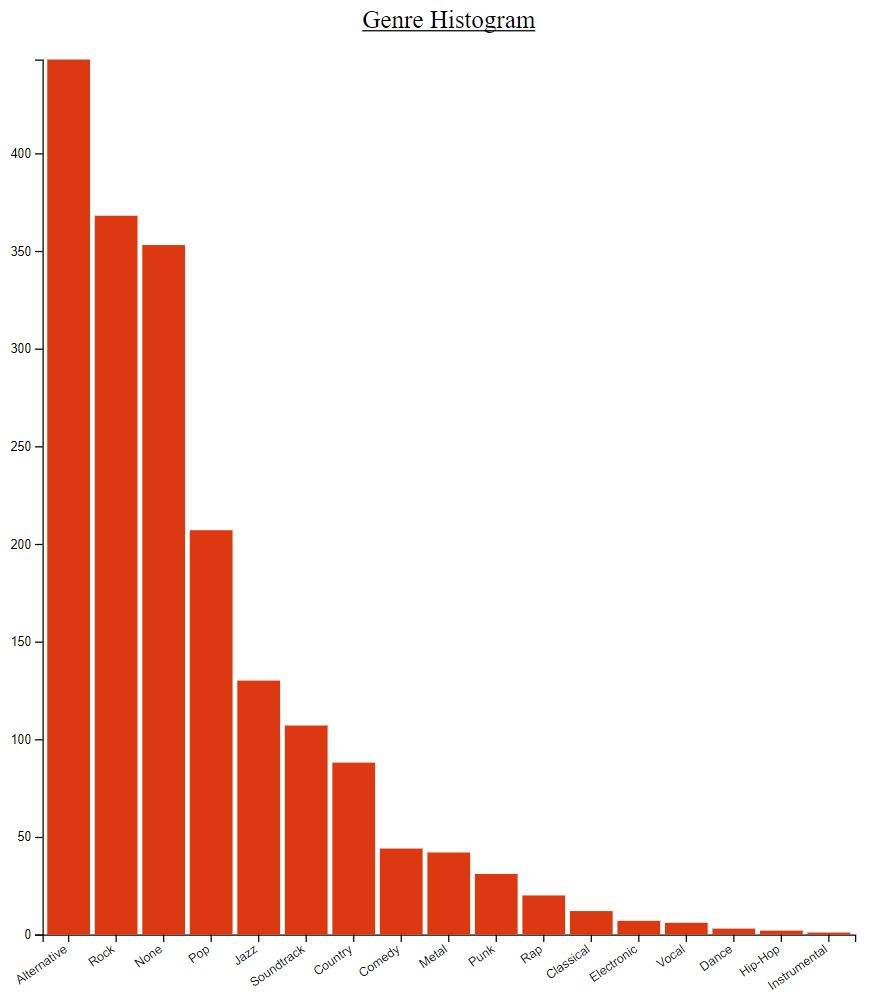
\includegraphics[width=\columnwidth]{genre-histogram}
 \caption{A genre histogram from \cite{Grifski:2019} of all the files in the dataset.}
 \label{fig:genres}
\end{figure}

The visualization in \autoref{fig:genres} was rendered from \autoref{tab:genres}
which contains 17 distinct genres including a placeholder for songs that have
no documented genre.

\begin{table}[h]
  \caption{Genre Totals}
  \label{tab:genres}
  \scriptsize%
	\centering%
  \begin{tabu}{l c}
  \toprule
    Genre & Count \\
  \midrule
    Alternative & 448 \\
    Rock & 368 \\
    None & 353 \\
    Pop & 207 \\
    Jazz & 130 \\
    Soundtrack & 107 \\
    Country & 88 \\
    Comedy & 44 \\
    Metal & 42 \\
    Punk & 31 \\
    Rap & 20 \\
    Classical & 12 \\
    Electronic & 7 \\
    Vocal & 6 \\
    Dance & 3 \\
    Hip-Hop & 2 \\
    Instrumental & 1 \\
  \midrule
    Sum & 1869 \\
  \bottomrule
  \end{tabu}%
\end{table}

To encode genres in later plots, I chose to use color. Unfortunately, D3 no
longer supports color pallets larger than 12 distinct colors, so I was forced
to filter the data set by the 12 most frequent genres in the dataset. As a
result, all following plots contain only the genres contained in
\autoref{tab:genres_filtered}.

\begin{table}[h]
  \caption{Filtered Genre Totals}
  \label{tab:genres_filtered}
  \scriptsize%
	\centering%
  \begin{tabu}{l c}
  \toprule
    Genre & Count \\
  \midrule
    Alternative & 448 \\
    Rock & 368 \\
    Pop & 207 \\
    Jazz & 130 \\
    Soundtrack & 107 \\
    Country & 88 \\
    Comedy & 44 \\
    Metal & 42 \\
    Punk & 31 \\
    Rap & 20 \\
    Classical & 12 \\
    Electronic & 7 \\
  \midrule
    Sum & 1504 \\
  \bottomrule
  \end{tabu}%
\end{table}

Since songs lacking genre data provide no useful insight in a genre comparative
study, I chose to exclude all files with None tags for genre. In total, I had
about 1,500 music files for visualization purposes.

\subsection{Duration Versus Release Date}

With a proper head count of genres and files, I proceeded to render a
visualization of duration by release date which can be seen in
\autoref{fig:duration}. After all, I was interested to see if song durations
have changed over time.

\begin{figure}[h]
 \centering % avoid the use of \begin{center}...\end{center} and use \centering instead (more compact)
 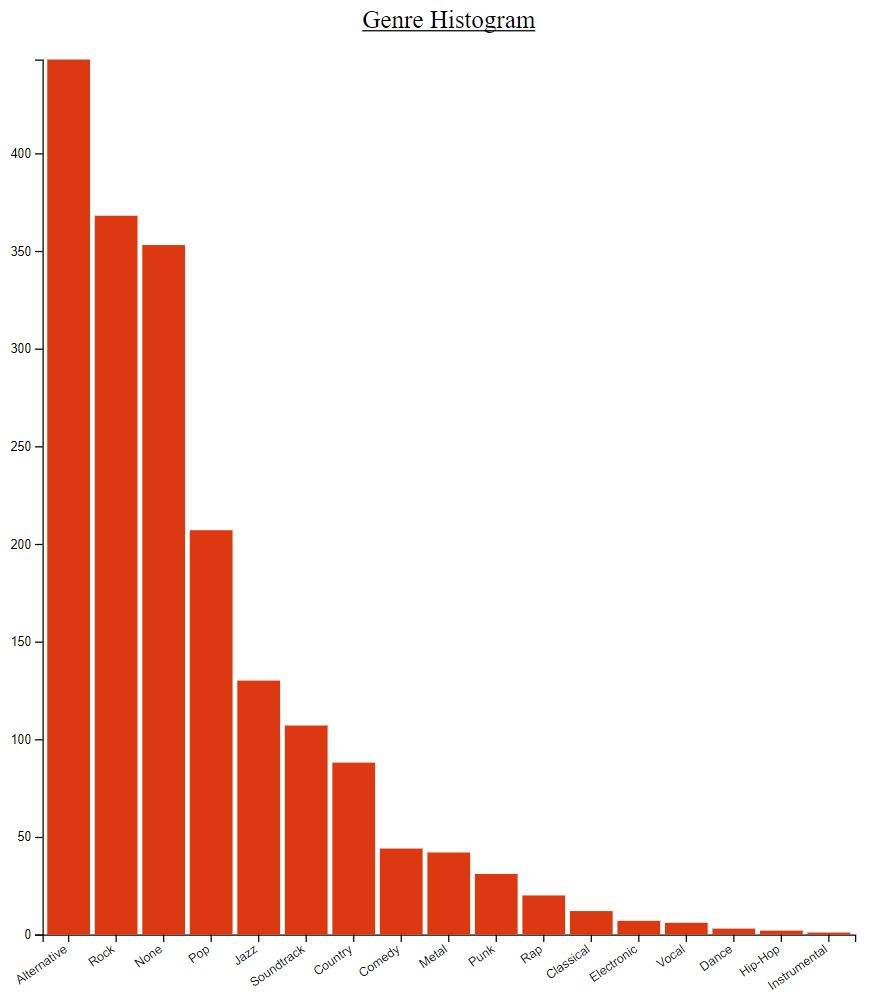
\includegraphics[width=\columnwidth]{genre-histogram}
 \caption{A genre histogram from \cite{Grifski:2019} of all the files in the dataset.}
 \label{fig:duration}
\end{figure}

Right away, it's clear which genres tend to have the longest durations. For
example, Metal and Classical music look like outliers with their durations
almost three times as long as what appears to be the average duration.

\subsection{dBFS Versus Release Date}

Since I was on the subject of data over time, I thought it would be interesting
to look at loudness over time using decibels at full scale (dBFS) and release
date. The ideas here being that songs may have changed in average loudness over
time. Naturally, the dBFS versus release data plot can be seen in
\autoref{fig:dBFS}.

\begin{figure}[h]
 \centering % avoid the use of \begin{center}...\end{center} and use \centering instead (more compact)
 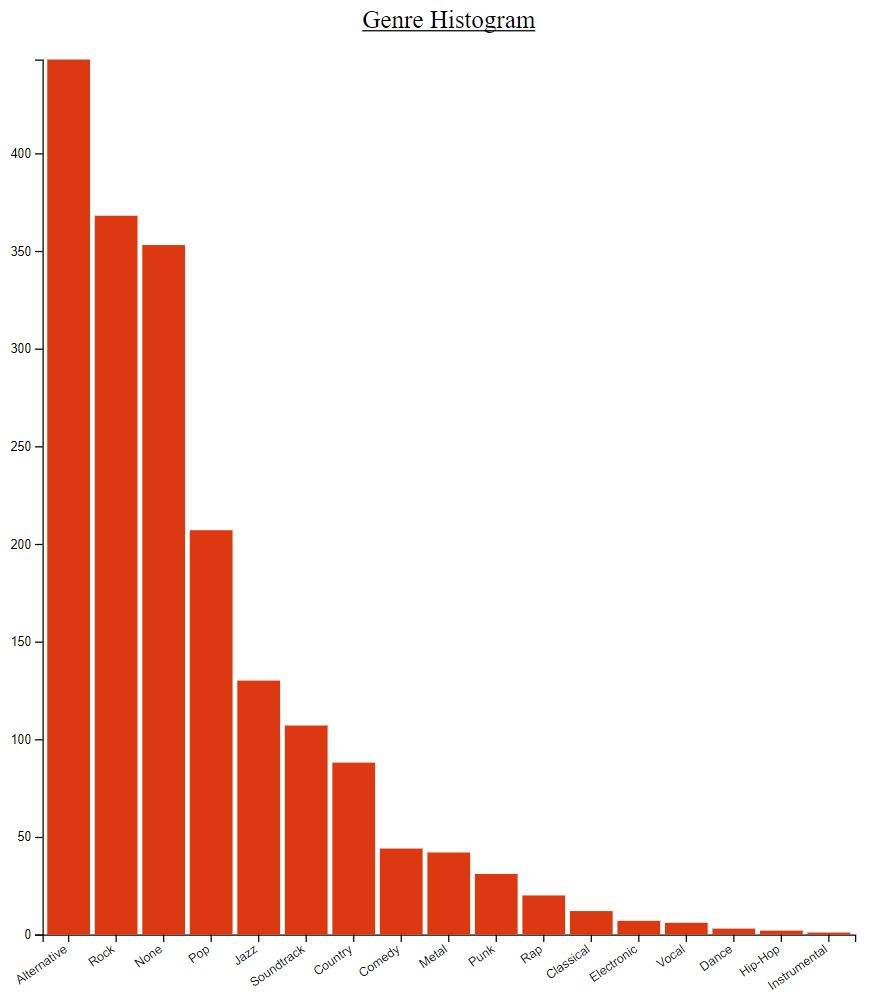
\includegraphics[width=\columnwidth]{genre-histogram}
 \caption{A genre histogram from \cite{Grifski:2019} of all the files in the dataset.}
 \label{fig:dBFS}
\end{figure}

After looking at \autoref{fig:dBFS}, it's tough to make a conclusion on any
trends in loudness over time. However, there are a few key features to notice.
For one, loudness appears to be trending up slightly. However, the loudness
is definitely more spread now than it used to be. In general, it seems songs
used to hover between -12 and -22 dBFS. Now, songs range anywhere from -8 to -26
dBFS.

In terms of genre, there are a lot of interesting trends. For example, Rock
is very clearly trending up in loudness. In the 70s, rock could be seen between
-14 and -24 dBFS. Now, rock can be seen at -14 in its quietest. Likewise,
genres like alternative and metal appear to be relatively loud on average.
Meanwhile, the soundtrack genre tends to be very quiet.

\subsection{Average dBFS Versus Genre}

Having seen an overview of dBFS over time, I had to take the analysis one step
further by asking: what genres are loudest on average? To do that, I ran an
analysis which captured the average dBFS of each genre and plotted on a bar
graph similar to the genre histogram.

\section{Challenges}

As it turns out, the scope of the initial proposal was much too broad. Many of
the signal processing approaches proposed were outside of my capabilities within
a semester. Given more time, I would have liked to explore audio features beyond
loudness such as pitch and onset.

\section{Conclusion}

After exploring M4A file parsing, audio signal processing, and genre data
visualization, I have concluded that analyzing music is a very difficult task.
While I had plenty of data, parsing common file formats, analyzing audio levels,
and generating compelling visualizations are not easy tasks.

That said, I learned a lot about the relationships between different genres
of music. For example, it's hardly surprising that certain genres have
longer songs on average (i.e. Jazz, Classical, and Metal). However, I was
suprised to see that songs have gotten slightly shorter over time.

In the future, I'd like to explore music genres with an even larger data set as
to avoid introducing any personal biases.

%\bibliographystyle{abbrv}
\bibliographystyle{abbrv-doi}
%\bibliographystyle{abbrv-doi-narrow}
%\bibliographystyle{abbrv-doi-hyperref}
%\bibliographystyle{abbrv-doi-hyperref-narrow}

\bibliography{report}
\end{document}
